\documentclass[a4paper,12pt]{jarticle}
\input ./chap01_preamble.tex
\graphicspath{%
  {../text01-img/}%
}
% !TEX root = ./chap01_03.tex
\begin{document}
\section[ラズベリーパイになれよう(2)]{ラズベリーパイになれよう(2)}
\subsection{写真をさつえいしよう}
\refstepcounter{Exercise}
\subsection{\theExercise ウェブカメラで写真をさつえいしよう}
\addtocounter{Exercise}{-1}\refstepcounter{Exercise}\label{E:webcam}
ウェブカメラを使用して\ruby{画像}{がぞう}をさつえいをします。

まずは、ラズベリーパイにウェブカメラを\ruby{接続}{せつぞく}しましょう。マウスと同じように、ウェブカメラのUSBのたんしをラズベリーパイのUSBたんしへ差し\ruby{込}{こ}みます。



\begin{figure}[ht]
  \centering
  \begin{minipage}{8.528cm}
    {\upshape
      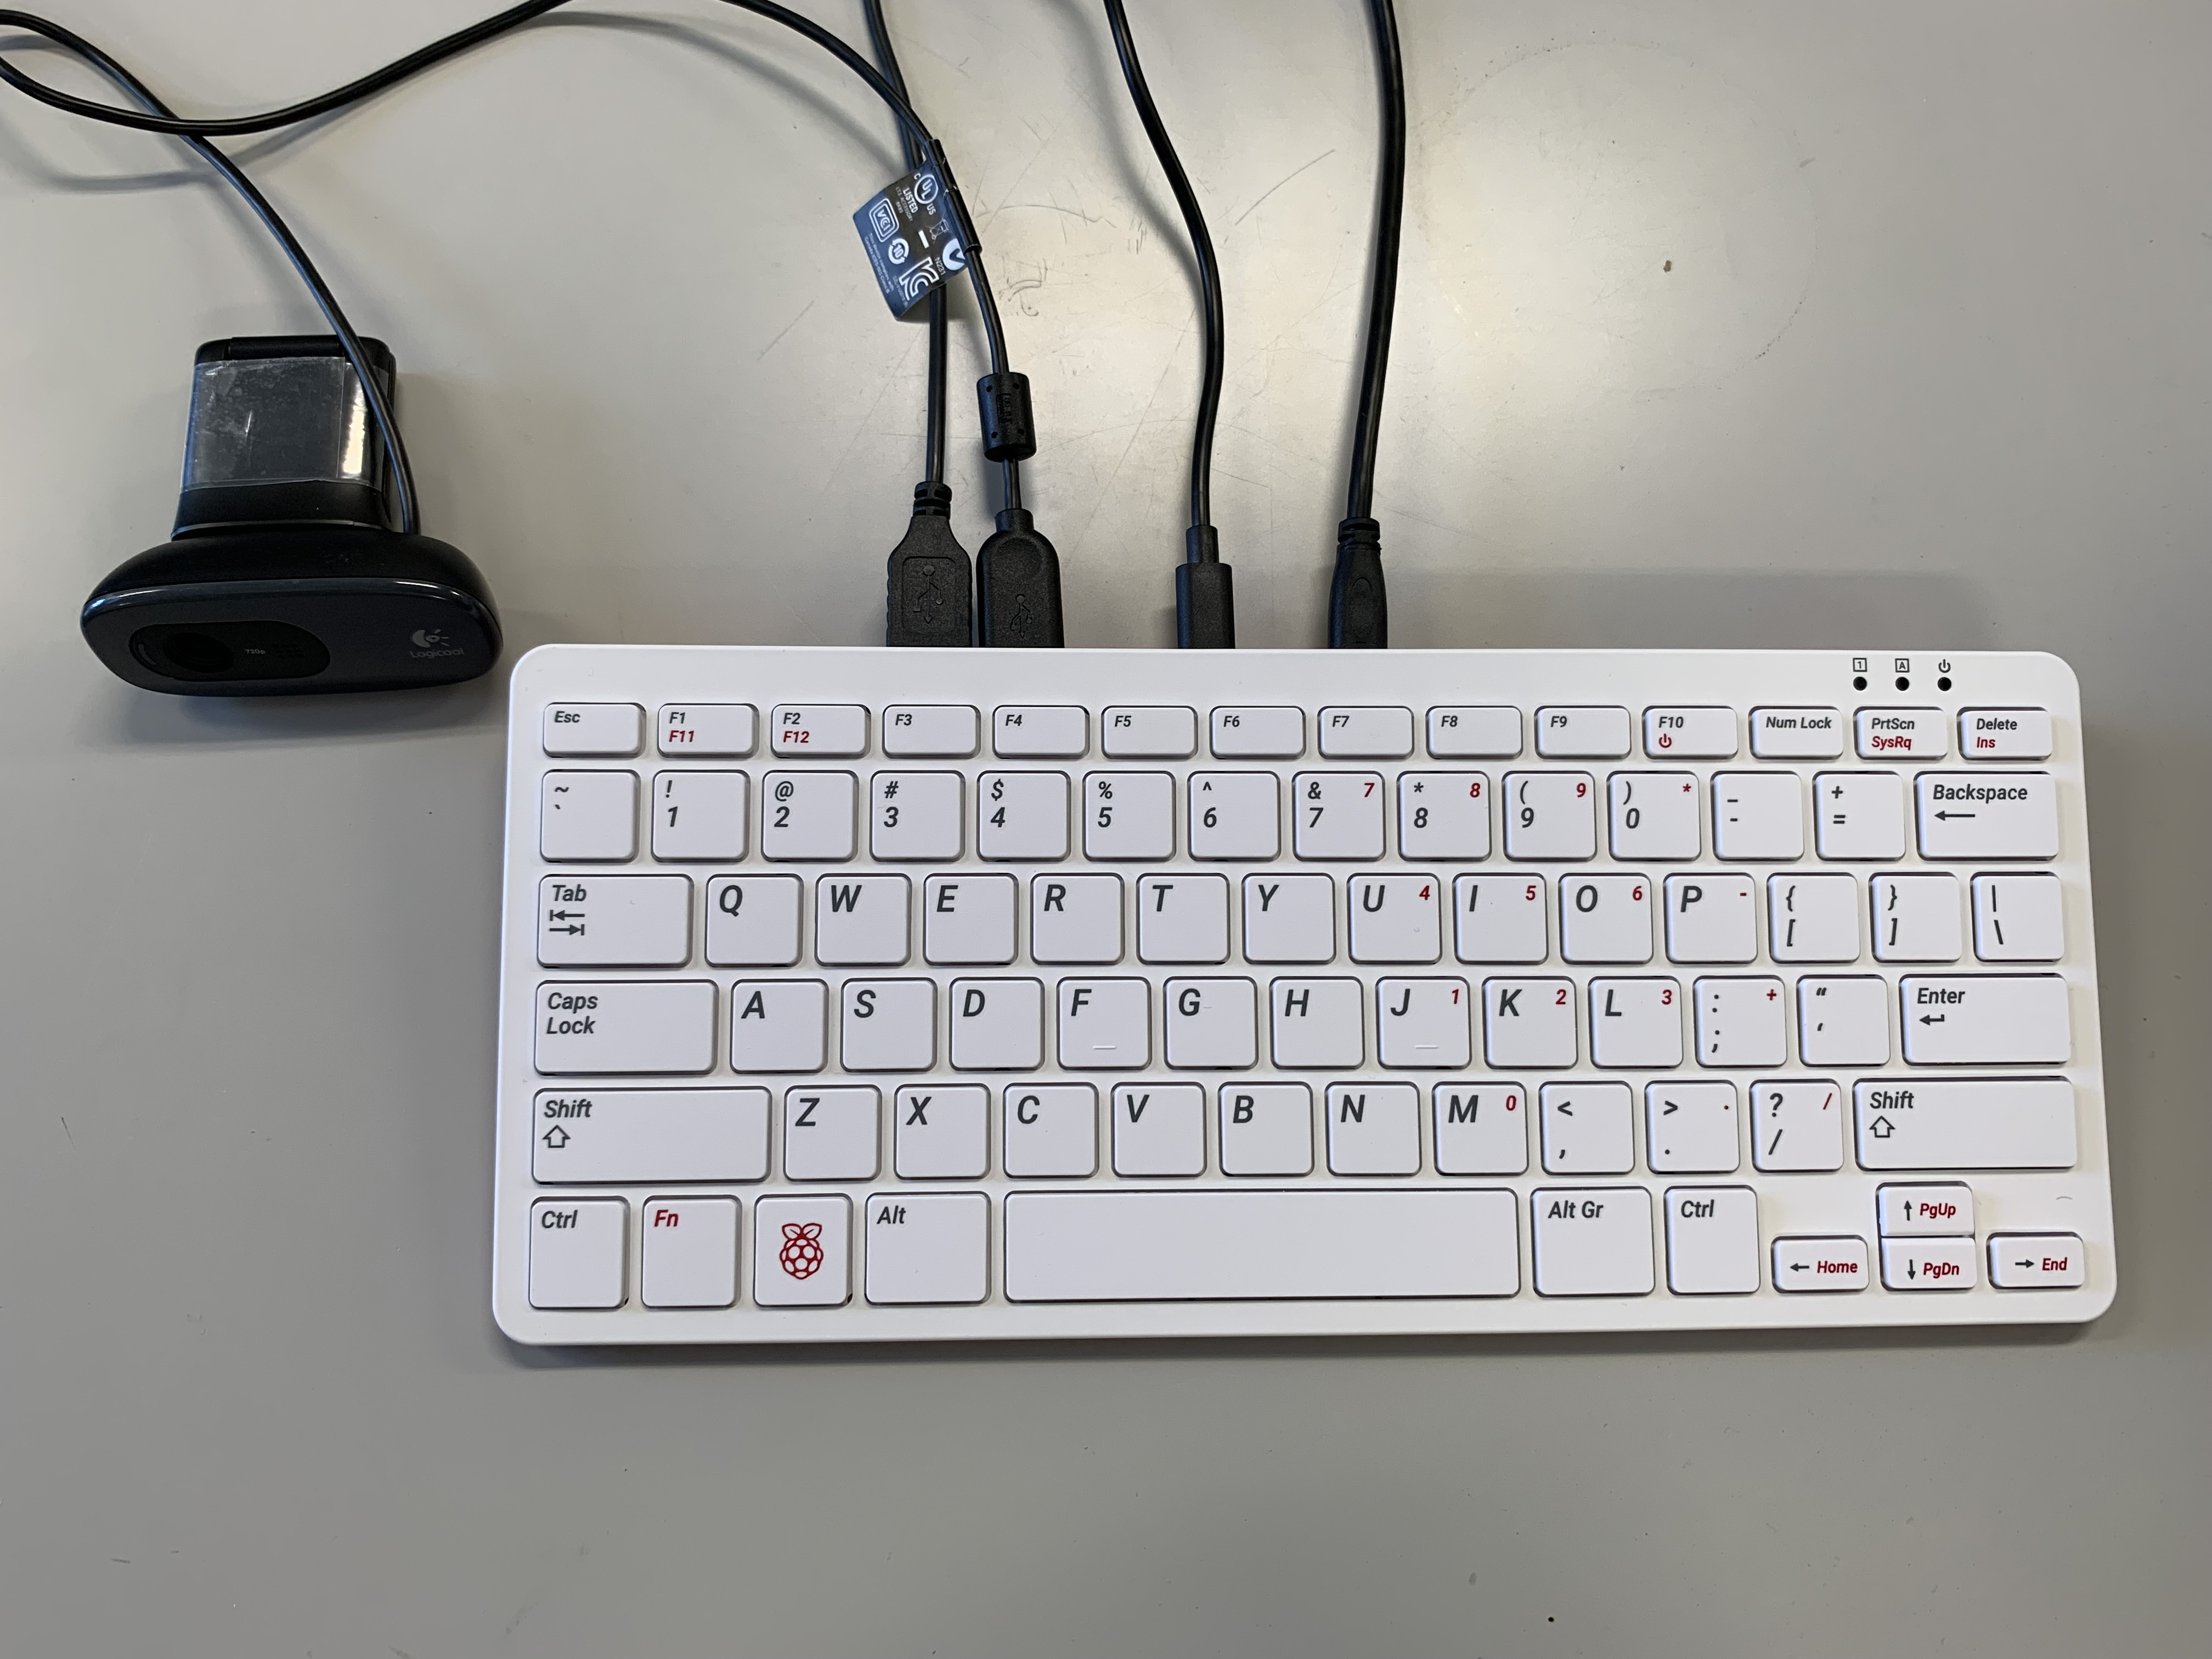
\includegraphics[width=7.904cm]{textbook-img112-2023.jpg}
      \newline
      \stepcounter{Figure}{\theFigure}: Webカメラの\ruby{接続}{せつぞく}}
  \end{minipage}
\end{figure}
ウェブカメラを\ruby{接続}{せつぞく}したら、ラズベリーパイからウェブカメラの\ruby{画像}{がぞう}を取得してみましょう。左上のラズベリーのアイコンをクリックします。そこから、サウンドとメディアを\ruby{選択}{せんたく}しVLCメディアプレーヤーをクリックします。

\begin{figure}[hb]
  \centering
  \begin{minipage}{10.917cm}
    {\upshape
      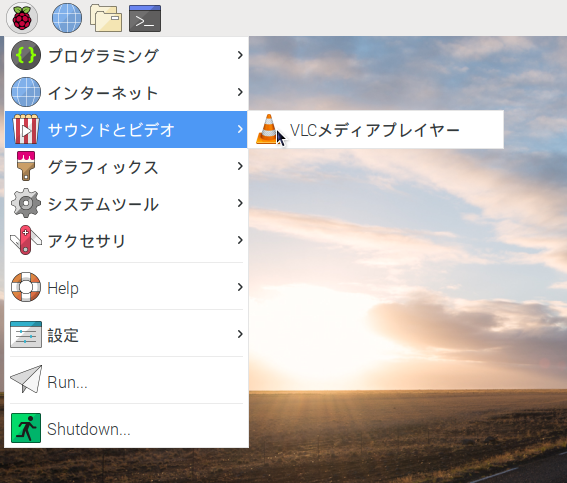
\includegraphics[height=8.715cm]{textbook-img113.png}
      \newline
      \stepcounter{Figure}{\theFigure}: メニューからVLC起動}
  \end{minipage}
\end{figure}
\clearpage
\begin{figure}[ht]
  ~\ref{seq:refFigure20}のようにVLCメディアプレーヤーが起動します。



  \centering
  \begin{minipage}{10cm}
    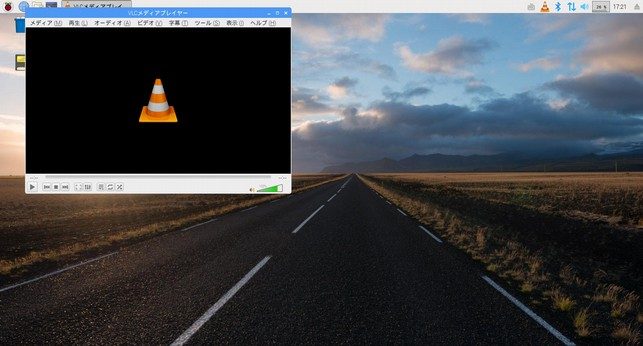
\includegraphics[width=10cm]{textbook-img114.jpg}


    {\refstepcounter{Figure}\theFigure\label{seq:refFigure20}}: VLC起動画面
  \end{minipage}
  \flushleft
  VLCが起動したら\ruby{確認}{かくにん}メッセージが出てきます。

  \textbf{\textcolor[rgb]{1.0,0.2,0.2}{赤わくで囲われているチェックボックスにチェックマーク(\CheckedBox)}}がついていないことを\ruby{確認}{かくにん}して続けるをクリックしてください。



  \centering
  \begin{minipage}{7.186cm}
    {\upshape
      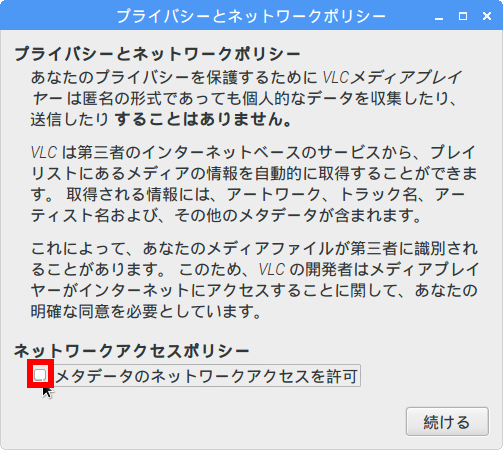
\includegraphics[width=7.2cm]{textbook-img115.png}
      \newline
      \stepcounter{Figure}{\theFigure}: \ruby{確認}{かくにん}メッセージ}
  \end{minipage}

  \flushleft
  カメラを開きます。~\ref{seq:refFigure22}のように\textbf{メディア}をクリックして\textbf{キャプチャーデバイスを開く}をクリックします。


  \centering
  \begin{minipage}{8.096cm}
    {\upshape
      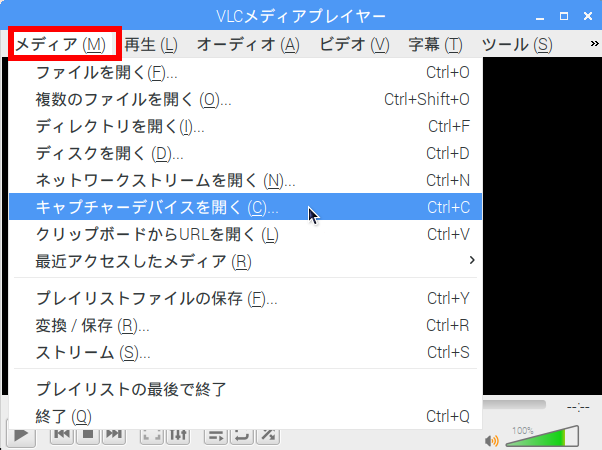
\includegraphics[width=8.0cm]{textbook-img116.png}
      \newline
      {\refstepcounter{Figure}\theFigure\label{seq:refFigure22}}:
      キャプチャデバイスをひらく}
  \end{minipage}
\end{figure}
\clearpage

\begin{figure}[ht]
  ~\ref{seq:refFigure23}のような画面がでてきます。
  赤線で囲われている\textbf{キャプチャーモード}を
  \textbf{Video camera}にして
  青線で囲われている\textbf{\ruby{再生}{さいせい}}をクリックします。


  \centering
  \begin{minipage}{10cm}
    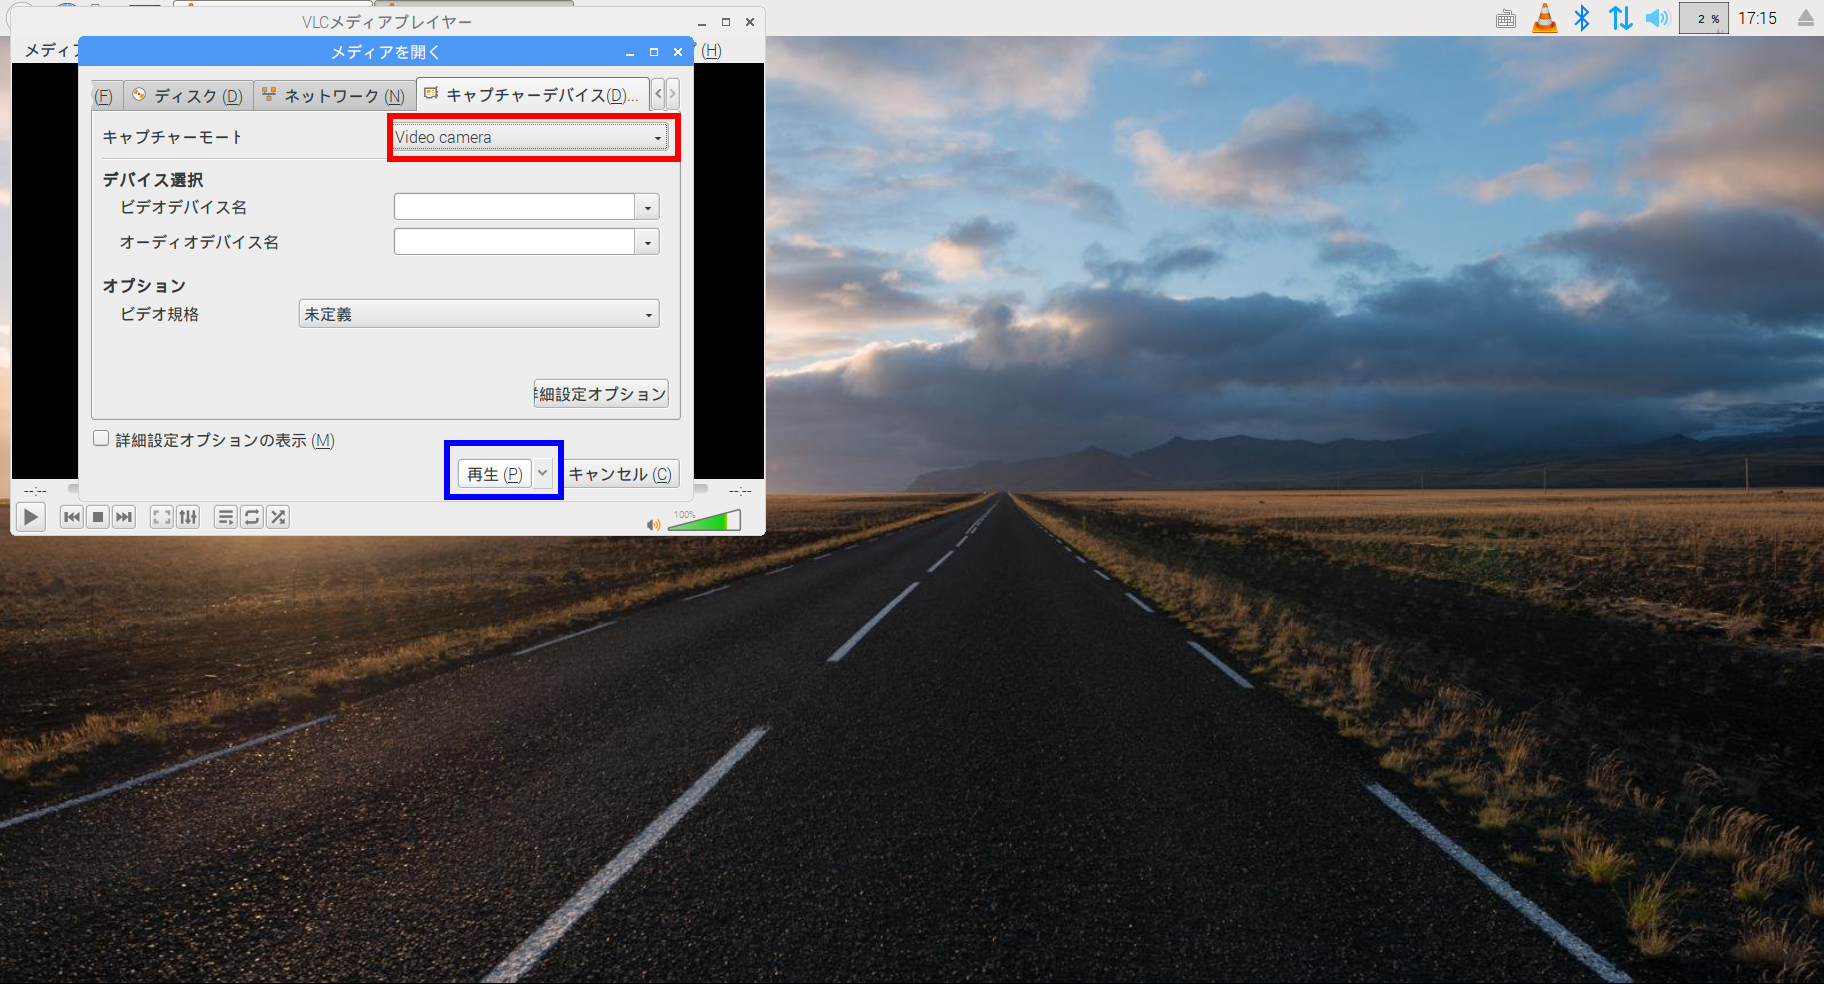
\includegraphics[width=10cm]{textbook-img117.png}
    {\refstepcounter{Figure}\theFigure\label{seq:refFigure23}}:
    キャプチャーデバイスを開く画面
  \end{minipage}

  \flushleft
  しばらくすると、カメラの\ruby{画像}{がぞう}が見えるようになります。

  \centering
  \begin{minipage}{10cm}
    {\upshape
      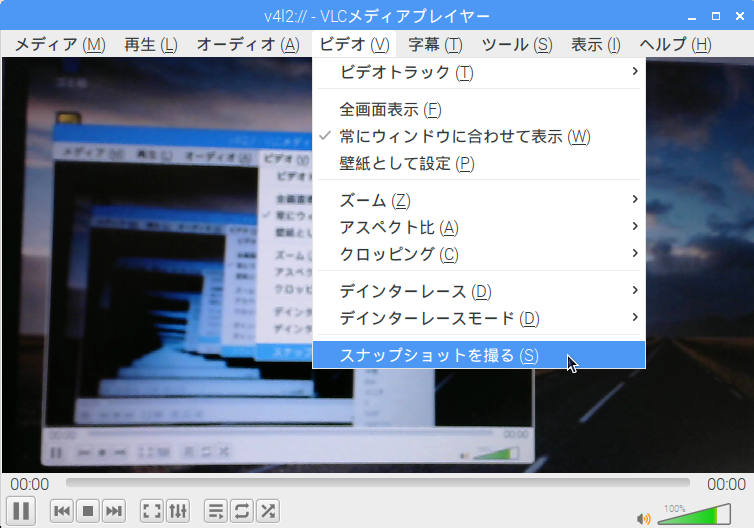
\includegraphics[width=10cm]{textbook-img118.png}
      \newline
      \stepcounter{Figure}{\theFigure}: スナップショット\ruby{撮影}{さつえい}}
  \end{minipage}
  \flushleft

  次に、カメラでさつえいしてみましょう。ビデオをクリックしてスナップショットを撮るをクリックします。


  \centering
  \begin{minipage}{10cm}
    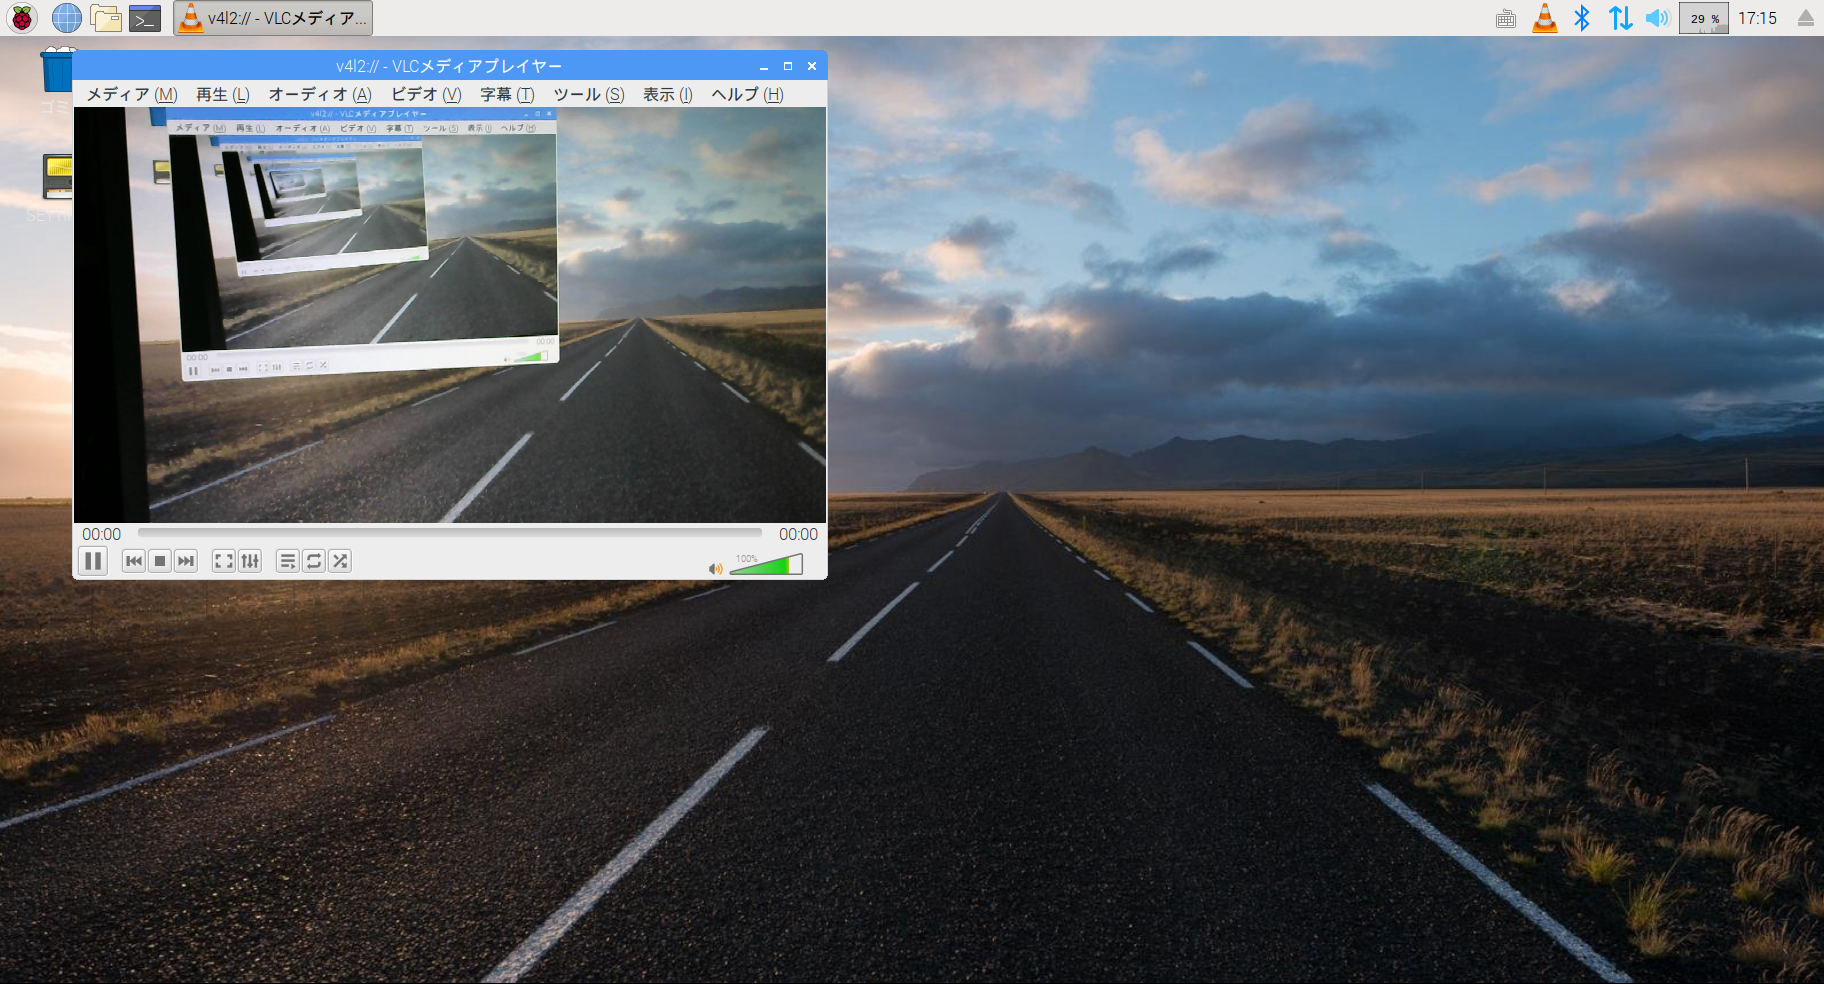
\includegraphics[width=10cm]{textbook-img119.png}
    {\upshape
      \stepcounter{Figure}{\theFigure}: カメラ入力}
  \end{minipage}
\end{figure}
\clearpage
\begin{figure}
  黒線の四角に囲われたように\ruby{保存}{ほぞん}場所が表示され、そこへ\ruby{画像}{がぞう}が\ruby{保存}{ほぞん}されます。

  \centering
  \begin{minipage}{10cm}
    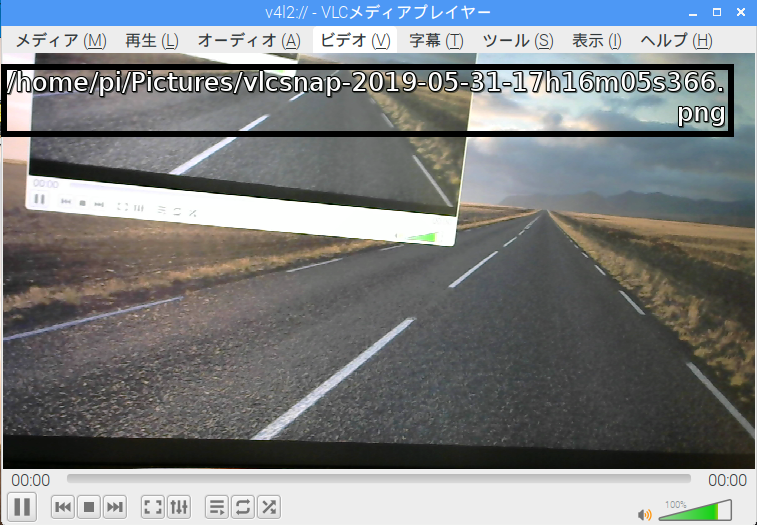
\includegraphics[width=10cm]{textbook-img120.png}
    \stepcounter{Figure}{\theFigure}: スナップショット\ruby{保存}{ほぞん}
  \end{minipage}



  \bigskip
  \flushleft

  初期\ruby{状態}{じょうたい}ではPicturesの下に\ruby{保存}{ほぞん}されます。\ruby{確認}{かくにん}してみましょう。



  \centering
  \begin{minipage}{10cm}
    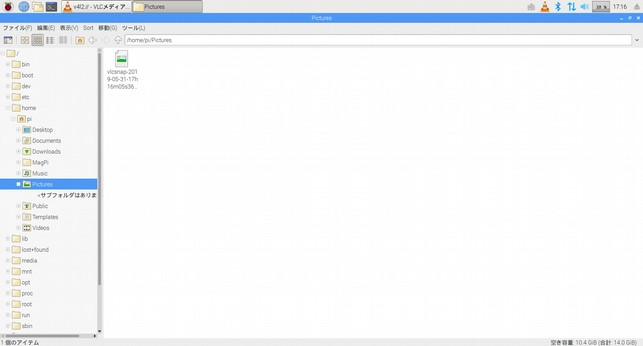
\includegraphics[width=10cm]{textbook-img121.jpg}

    \stepcounter{Figure}{\theFigure}: \ruby{画像}{がぞう}\ruby{撮影}{さつえい}場所
  \end{minipage}


  \bigskip

  \flushleft
  とった\ruby{画像}{がぞう}を\ruby{確認}{かくにん}してみましょう。~\ref{seq:refFigure28}の赤わくで囲ってあるものがとった写真です。ダブルクリックをすると、\ruby{画像}{がぞう}を開いて見ることができます。



  \centering
  \begin{minipage}{10cm}
    {\upshape
      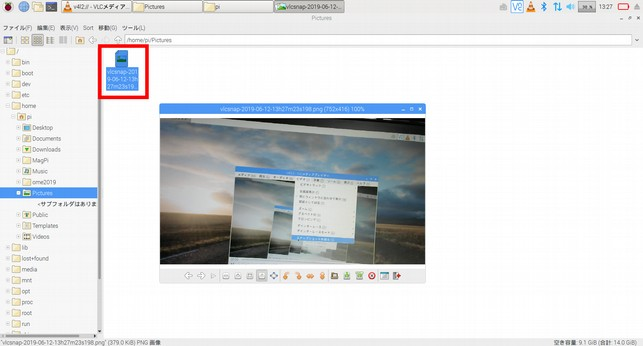
\includegraphics[width=10cm]{textbook-img122.jpg}
      \newline
      {\refstepcounter{Figure}\theFigure\label{seq:refFigure28}}:
      とった\ruby{画像}{がぞう}を開く}
  \end{minipage}
\end{figure}

\bigskip

\clearpage

\begin{figure}[ht]
  \refstepcounter{Exercise}
  \subsection{\theExercise \ruby{画像}{がぞう}に絵をかこう}

  \bigskip

  “GIMP”ソフトを立ち上げて、色付きの筆で自分の顔写真に絵をかこう

  \ruby{画像}{がぞう}を開いて、色を\ruby{選択}{せんたく}、お絵かきツールの筆を選んで書くよ

  \textbf{考え方}



  \begin{minipage}{\textwidth}
    \centering
    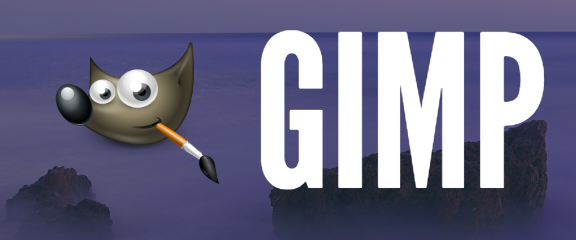
\includegraphics[width=6.112cm]{textbook-img123.png}
    \begin{minipage}[b]{8.617cm}

      本格的な\ruby{画像}{がぞう}\ruby{編集}{へんしゅう}、加工ソフトの

      GIMPを使って自分の顔写真などの

      \ruby{画像}{がぞう}を\ruby{編集}{へんしゅう}してみよう
    \end{minipage}


  \end{minipage}
  \bigskip




  \begin{minipage}{\textwidth}
    \centering
    \begin{minipage}{5.852cm}
      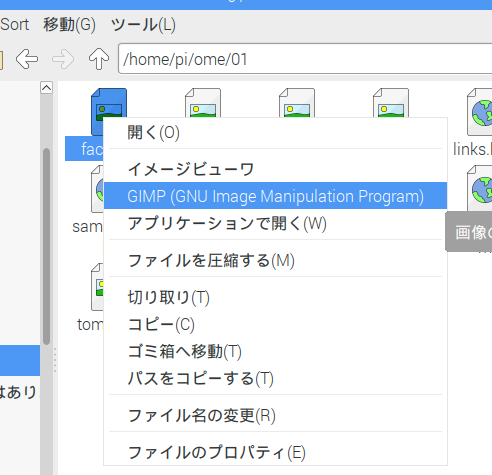
\includegraphics[width=5.359cm]{textbook-img124.png}\\
      1 \ruby{編集}{へんしゅう}したい\ruby{画像}{がぞう}ファイルを

      右クリックしGIMPをクリック
    \end{minipage}
    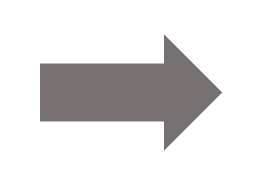
\includegraphics[width=1.489cm]{textbook-img128.png}
    \begin{minipage}{7.975cm}
      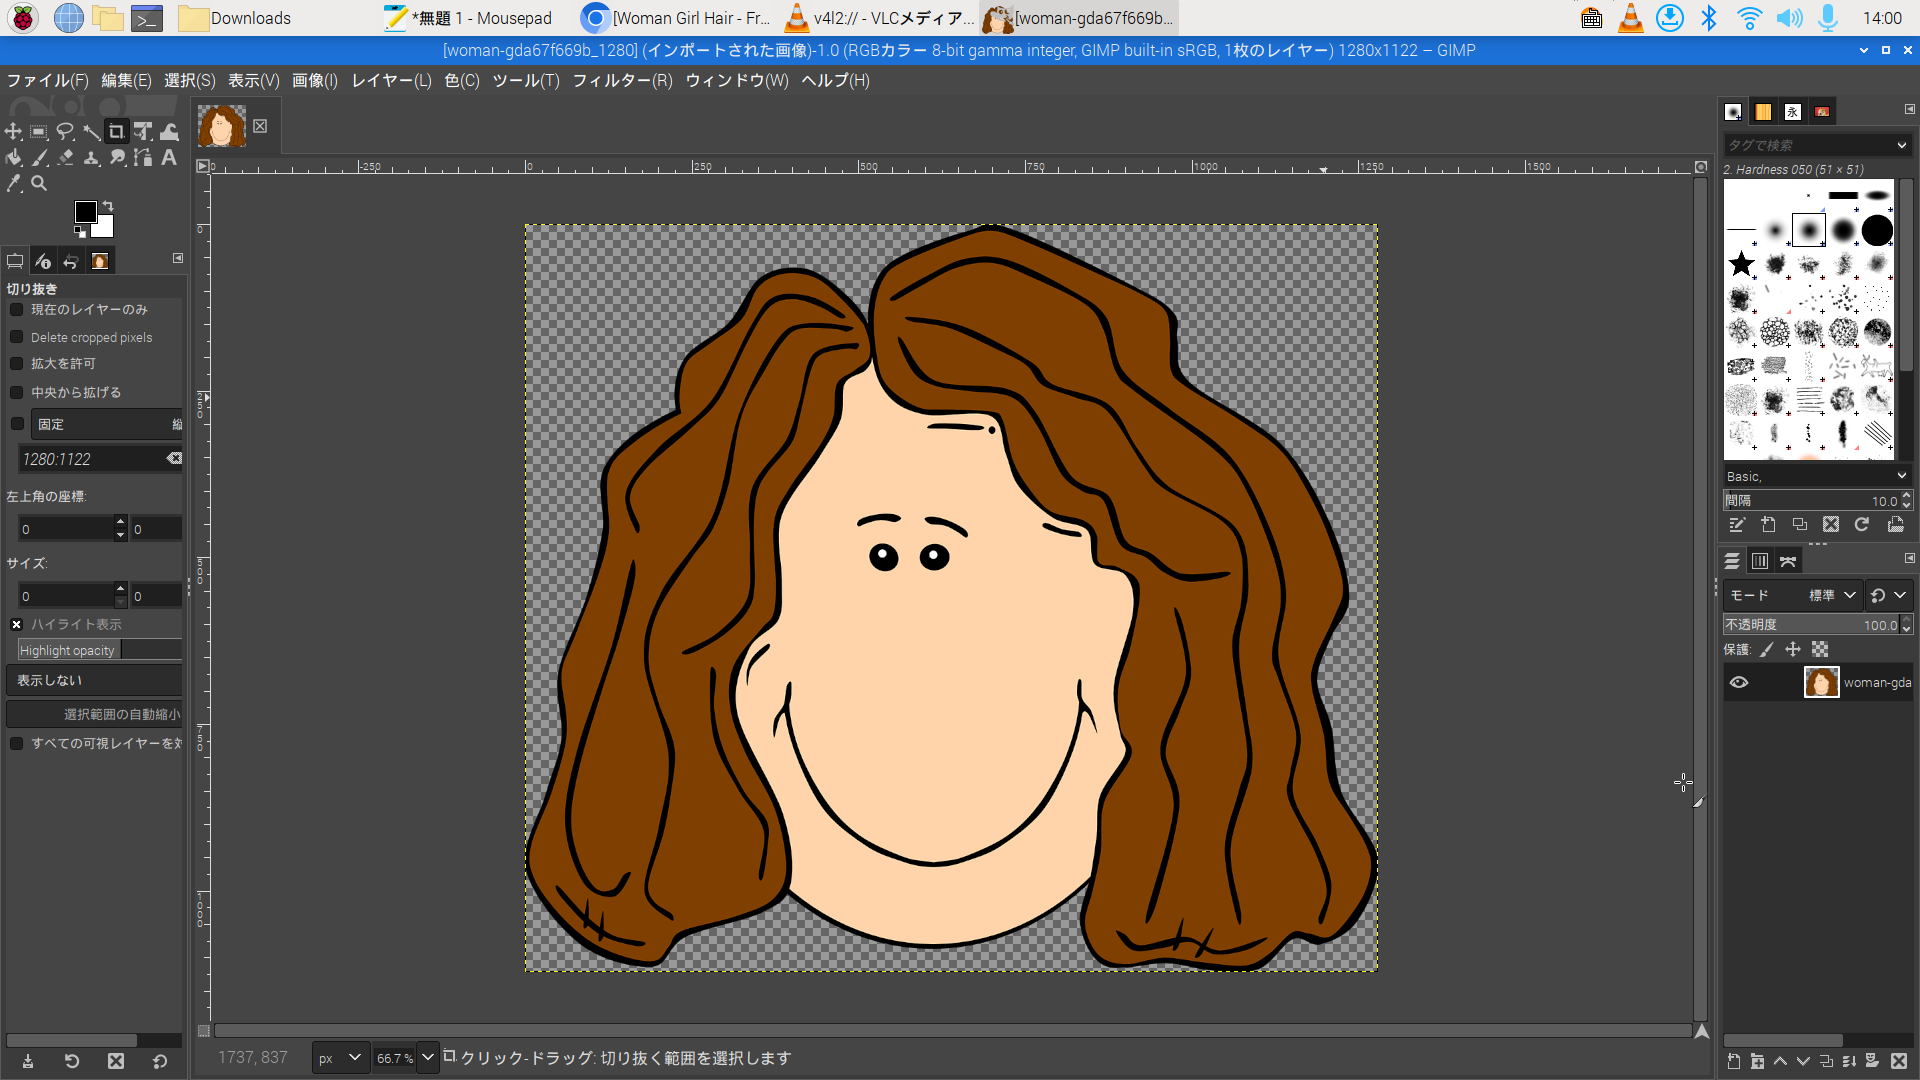
\includegraphics[width=7cm]{textbook-img125.png}\\
      2 \ruby{画像}{がぞう}\ruby{編集}{へんしゅう}モードになるよ
    \end{minipage}


  \end{minipage}
  \bigskip




  \begin{minipage}{\textwidth}
    \begin{minipage}{5.984cm}
      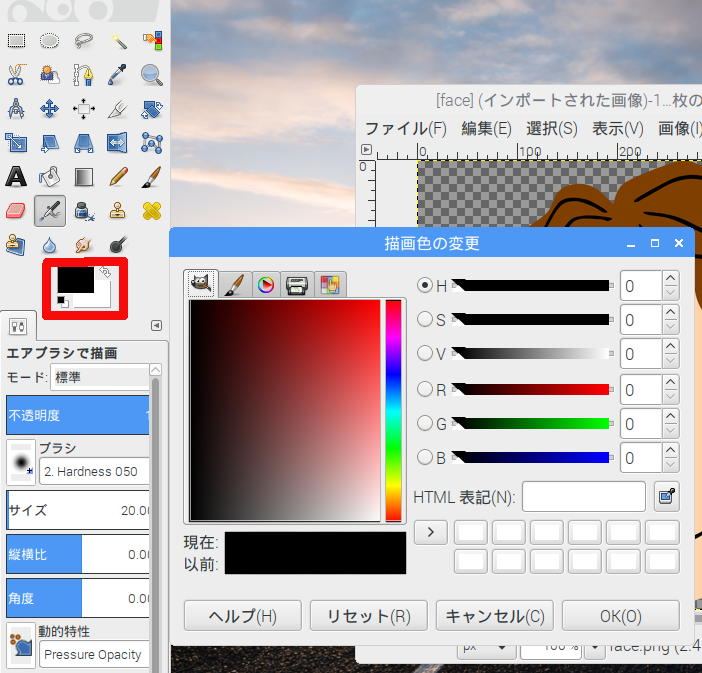
\includegraphics[width=5.971cm]{textbook-img129.png}\\
      3 赤い丸で囲まれている

      部分をクリック


      \bigskip
    \end{minipage}
    \hfill
    \begin{minipage}{8.984cm}
      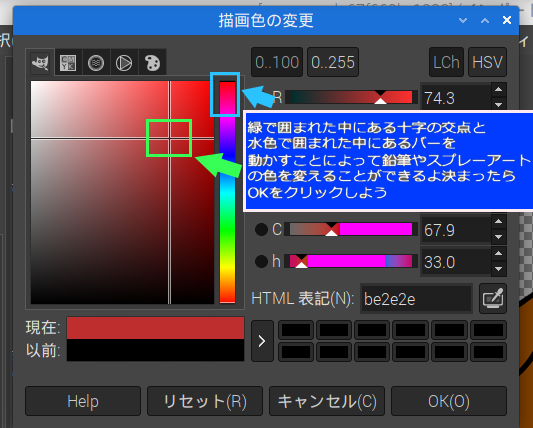
\includegraphics[width=7cm]{textbook-img126.png}\\
      4 色を変更しよう

      好きな色を選んでOKを\ruby{押}{お}します


      \bigskip
      \begin{minipage}{5.984cm}
        5
        今回は色を赤にしました。赤く囲んであるところの色が赤に変わっていることを\ruby{確認}{かくにん}してください。


      \end{minipage}
    \end{minipage}
  \end{minipage}

  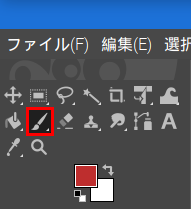
\includegraphics[width=1.866cm]{textbook-img127.png}
  \begin{minipage}[b]{6.663cm}
    6 次にお絵かきツールを選びます。

    赤色で囲われているところをクリックしてください。これで色付きの筆が使えるようになります。


    \bigskip

  \end{minipage}
\end{figure}
\clearpage
\begin{figure}[ht]
  \textbf{考え方(続き)}

  \begin{minipage}{\textwidth}
    \centering
    \begin{minipage}{5.76cm}
      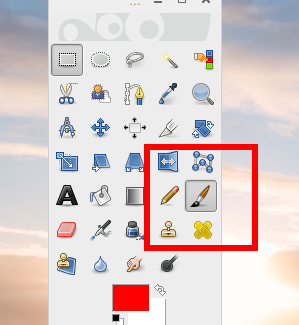
\includegraphics[width=5.05cm]{textbook-img130.png}\\
      7
      ツール\ruby{一覧}{いちらん}の下の文字が「ブラシで\ruby{描画}{びょうが}」に変わったことを\ruby{確認}{かくにん}しましょう。これで筆が使えるようになりました。
    \end{minipage}
    \hfill
    \begin{minipage}{10.2cm}
      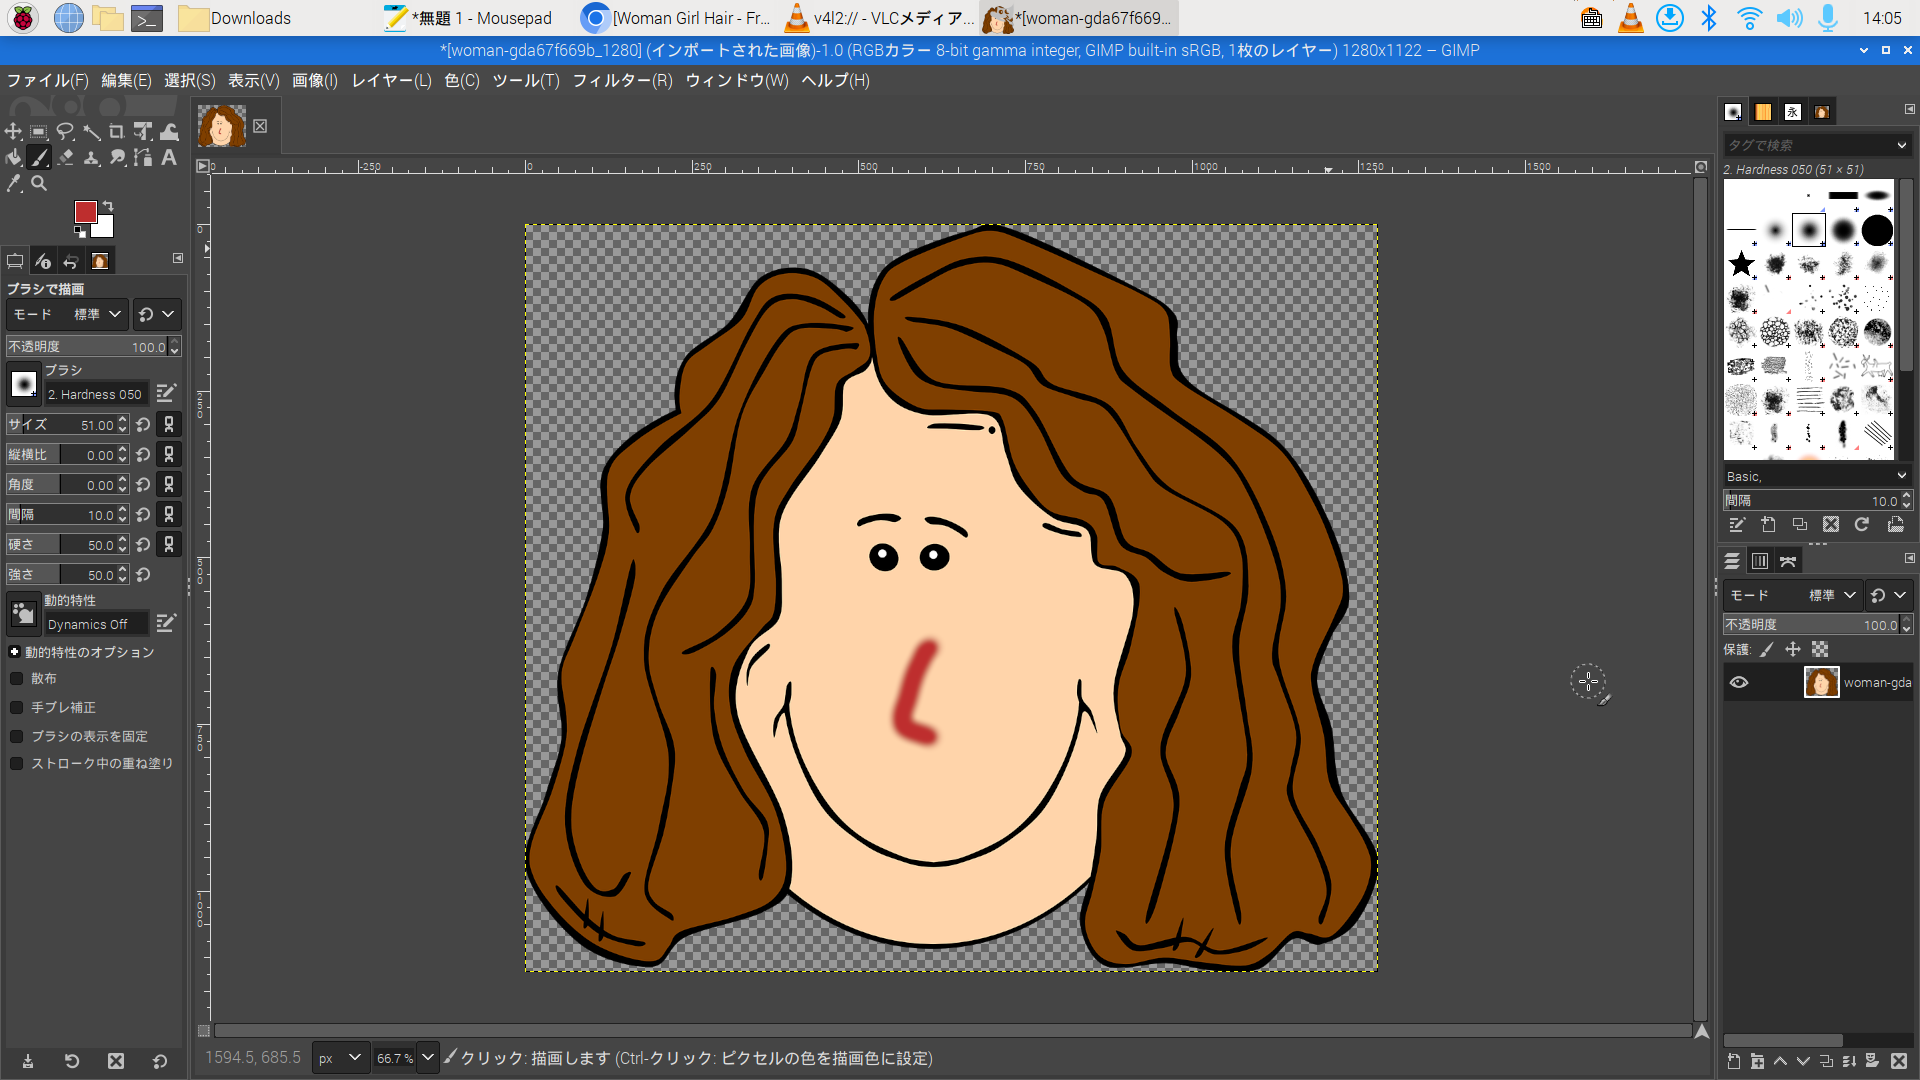
\includegraphics[width=10.134cm]{textbook-img131.png}\\
      8 左クリックをおしながら\ruby{画像}{がぞう}の上を\ruby{移動}{いどう}させると筆でお絵かきができます。いたずら書きをしてみてください
    \end{minipage}
  \end{minipage}


  \bigskip

  \begin{minipage}{\textwidth}
    \begin{minipage}{6.984cm}
      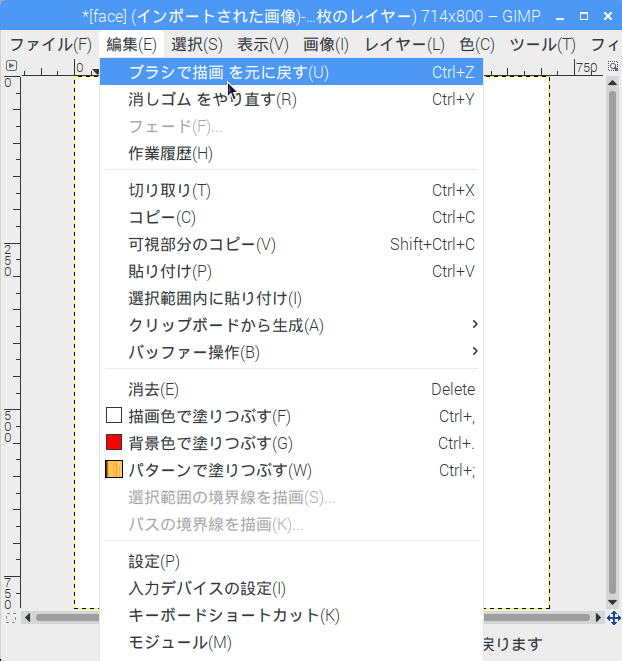
\includegraphics[width=6.228cm]{textbook-img132.png}\\
      9 \ruby{間違}{まちが}えてしまって、もとに\ruby{戻}{もど}したいとなったらメニューの\ruby{編集}{へんしゅう}からもとに\ruby{戻}{もど}すをクリックします。
    \end{minipage}
    \hfill
    \begin{minipage}{8.966cm}
      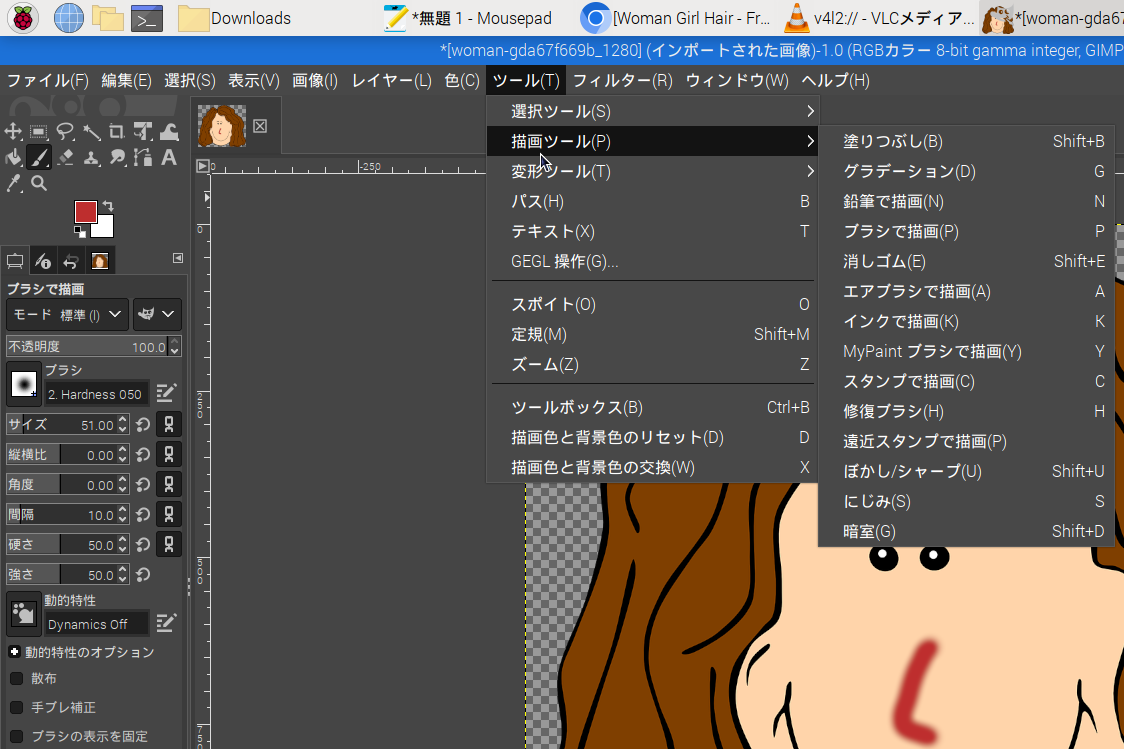
\includegraphics[width=8.881cm,height=4.997cm]{textbook-img133.png}\\
      10 他にもたくさんツールはあります。メニューのツール\ruby{欄}{らん}にある\ruby{描画}{びょうが}ツールで選べるよ。\ruby{鉛筆}{えんぴつ}、インクを試してみよう。書き方はいっしょで左クリックをを\ruby{押}{お}しながら\ruby{移動}{いどう}だよ
    \end{minipage}
  \end{minipage}
\end{figure}


\clearpage
\begin{figure}
  \textbf{考え方(続き)}


  \ruby{編集}{へんしゅう}しおわったら書き出しをします。

  \centering
  \begin{minipage}{\textwidth}
    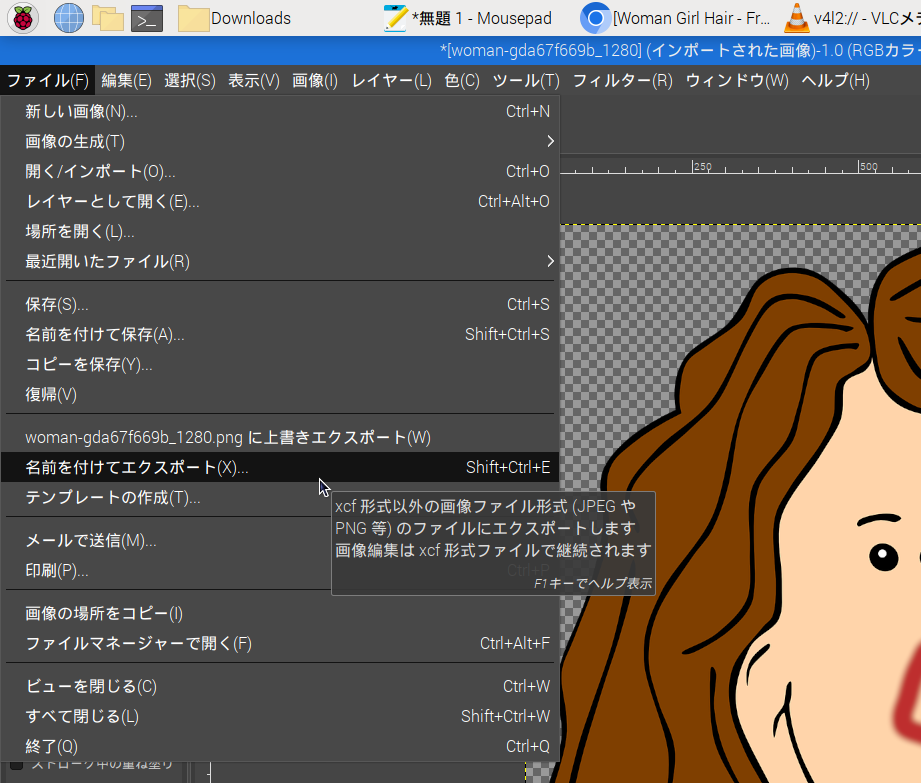
\includegraphics[width=0.5\textwidth]{textbook-img138.png}\\
    11 \ruby{編集}{へんしゅう}がおわったら

    ファイルから名前を付けてエクスポートをクリック
  \end{minipage}

  \bigskip


  \begin{minipage}{\textwidth}
    \begin{minipage}{0.45\textwidth}
      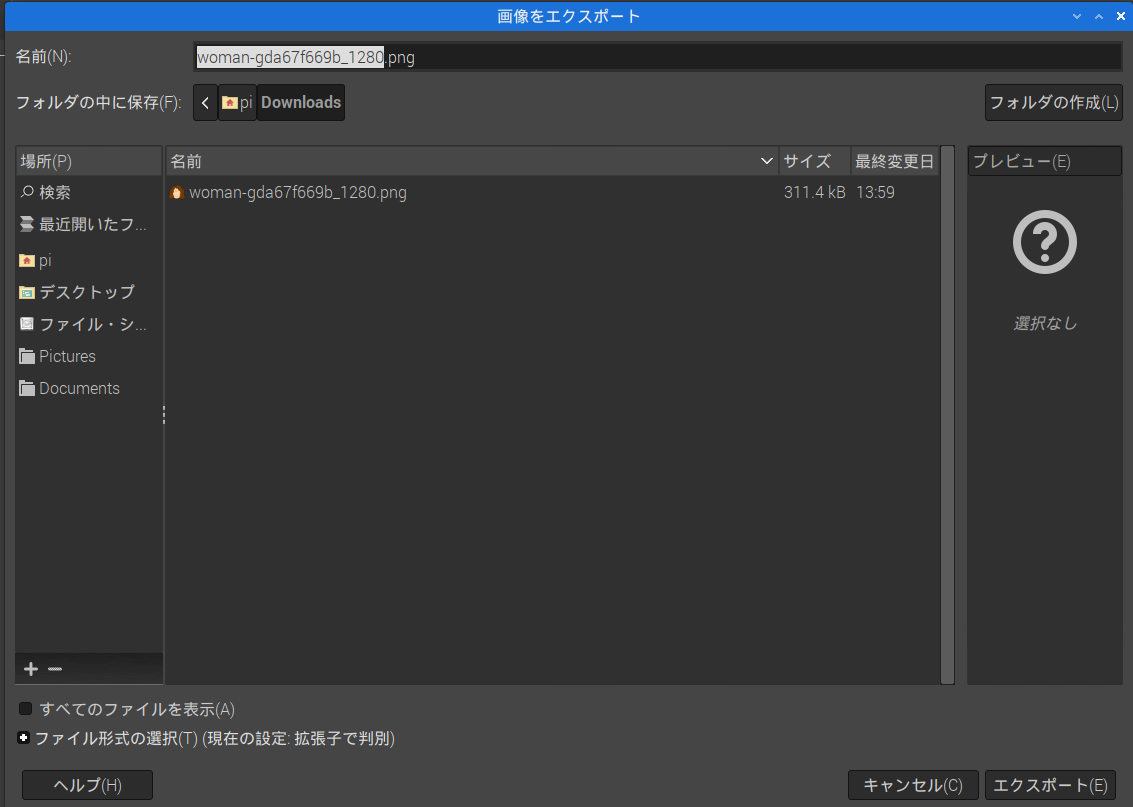
\includegraphics[width=\linewidth]{textbook-img137.png}\\
      12
      下のエクスポートをクリック(.jpegファイルから\ruby{編集}{へんしゅう}したならば12へ)
    \end{minipage}
    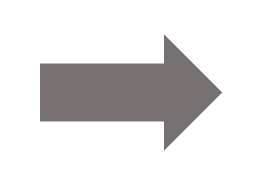
\includegraphics[width=1.919cm]{textbook-img135.png}
    \begin{minipage}{0.45\textwidth}
      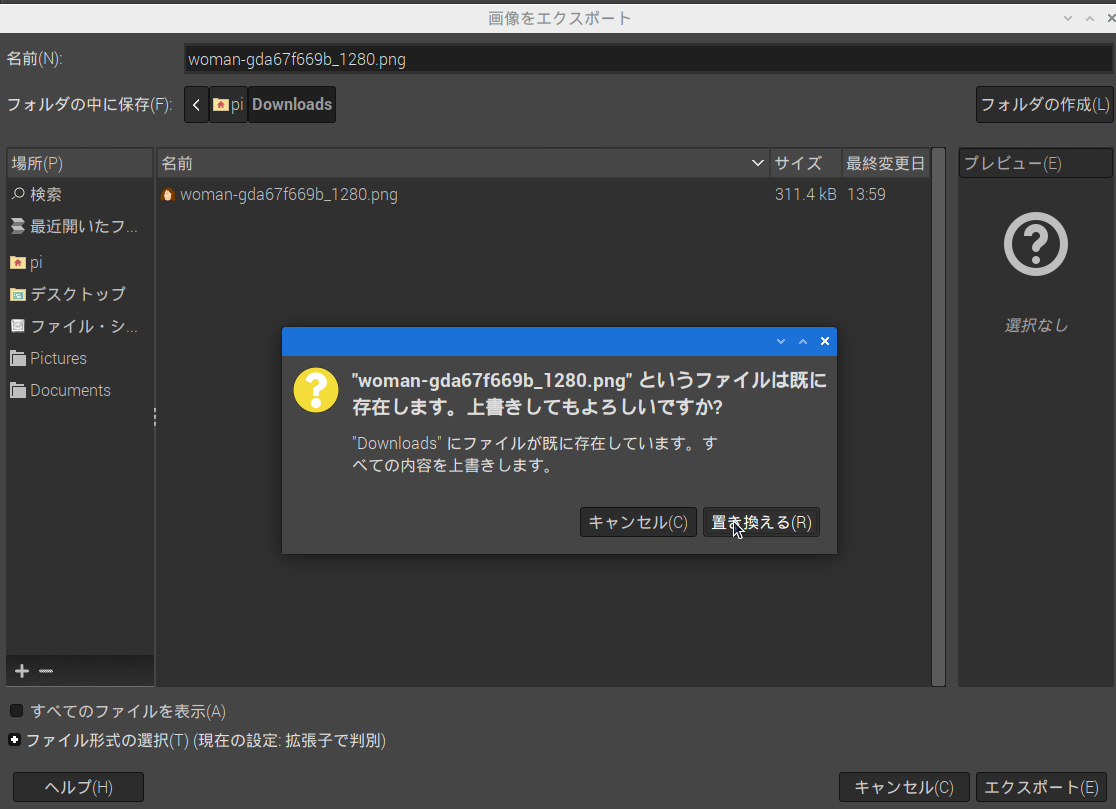
\includegraphics[width=\linewidth]{textbook-img136.png}\\
      13 置き換えるをクリック
    \end{minipage}
  \end{minipage}

  \bigskip


  \begin{minipage}{\textwidth}
    \begin{minipage}{0.45\textwidth}
      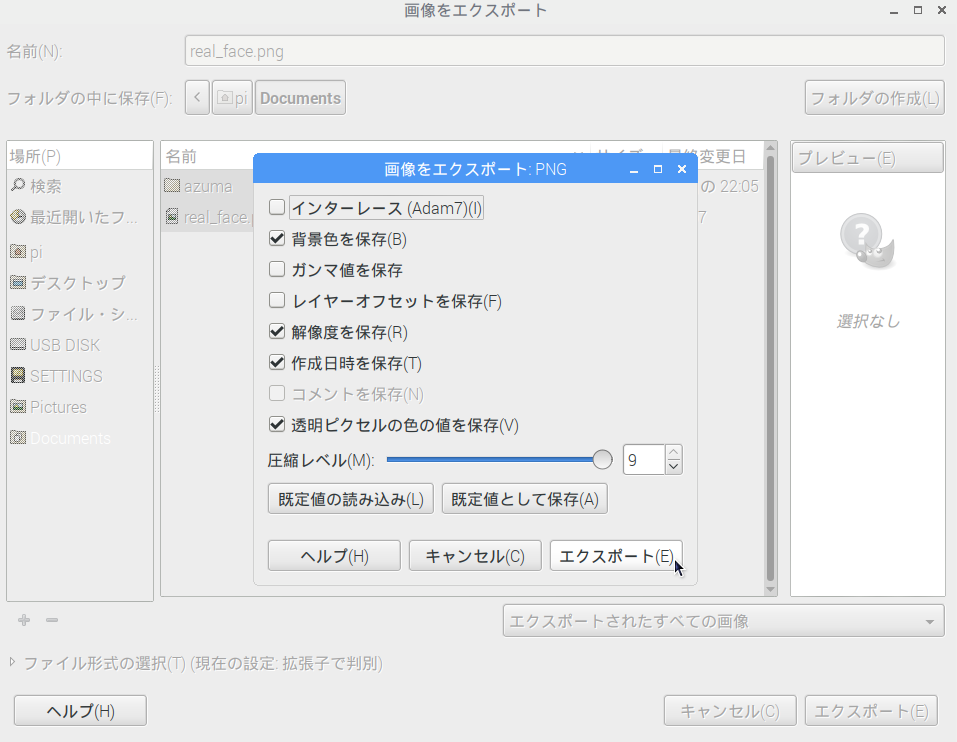
\includegraphics[width=\linewidth]{textbook-img134.png}\\
      14 エクスポートをクリック
    \end{minipage}
    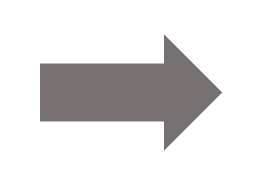
\includegraphics[width=1.919cm]{textbook-img135.png}
    \begin{minipage}{0.45\textwidth}
      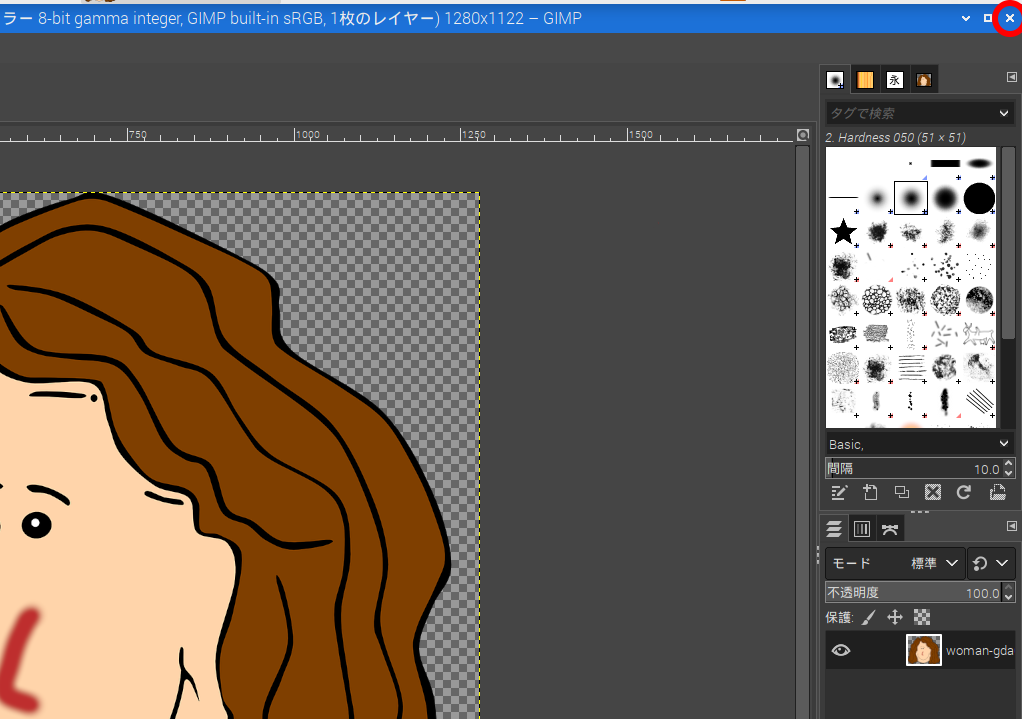
\includegraphics[width=\linewidth]{textbook-img1030.png}\\
      15
      右上の赤い丸で囲まれた×ボタンをを\ruby{押}{お}して、\ruby{画像}{がぞう}\ruby{編集}{へんしゅう}ツールを\ruby{閉}{と}じよう
    \end{minipage}
  \end{minipage}



\end{figure}
\clearpage

\begin{figure}
  \textbf{考え方(続き)}

  \begin{minipage}{\textwidth}
    \begin{minipage}{0.45\linewidth}
      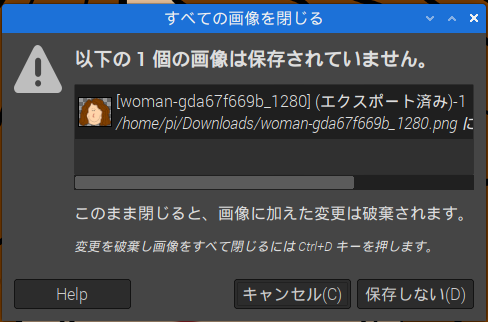
\includegraphics[width=\linewidth]{textbook-img1031.png}\\
      16 「\ruby{保存}{ほぞん}されていません」というウィンドウがでます。これは、先ほど「エクスポート」したものとは別のことを言っていて、
      \ruby{画像}{がぞう}自体は\ruby{保存}{ほぞん}されています。なので、気にせず「\ruby{保存}{ほぞん}しない」をクリックしましょう
    \end{minipage}
    \hfill
    \begin{minipage}{0.45\linewidth}
      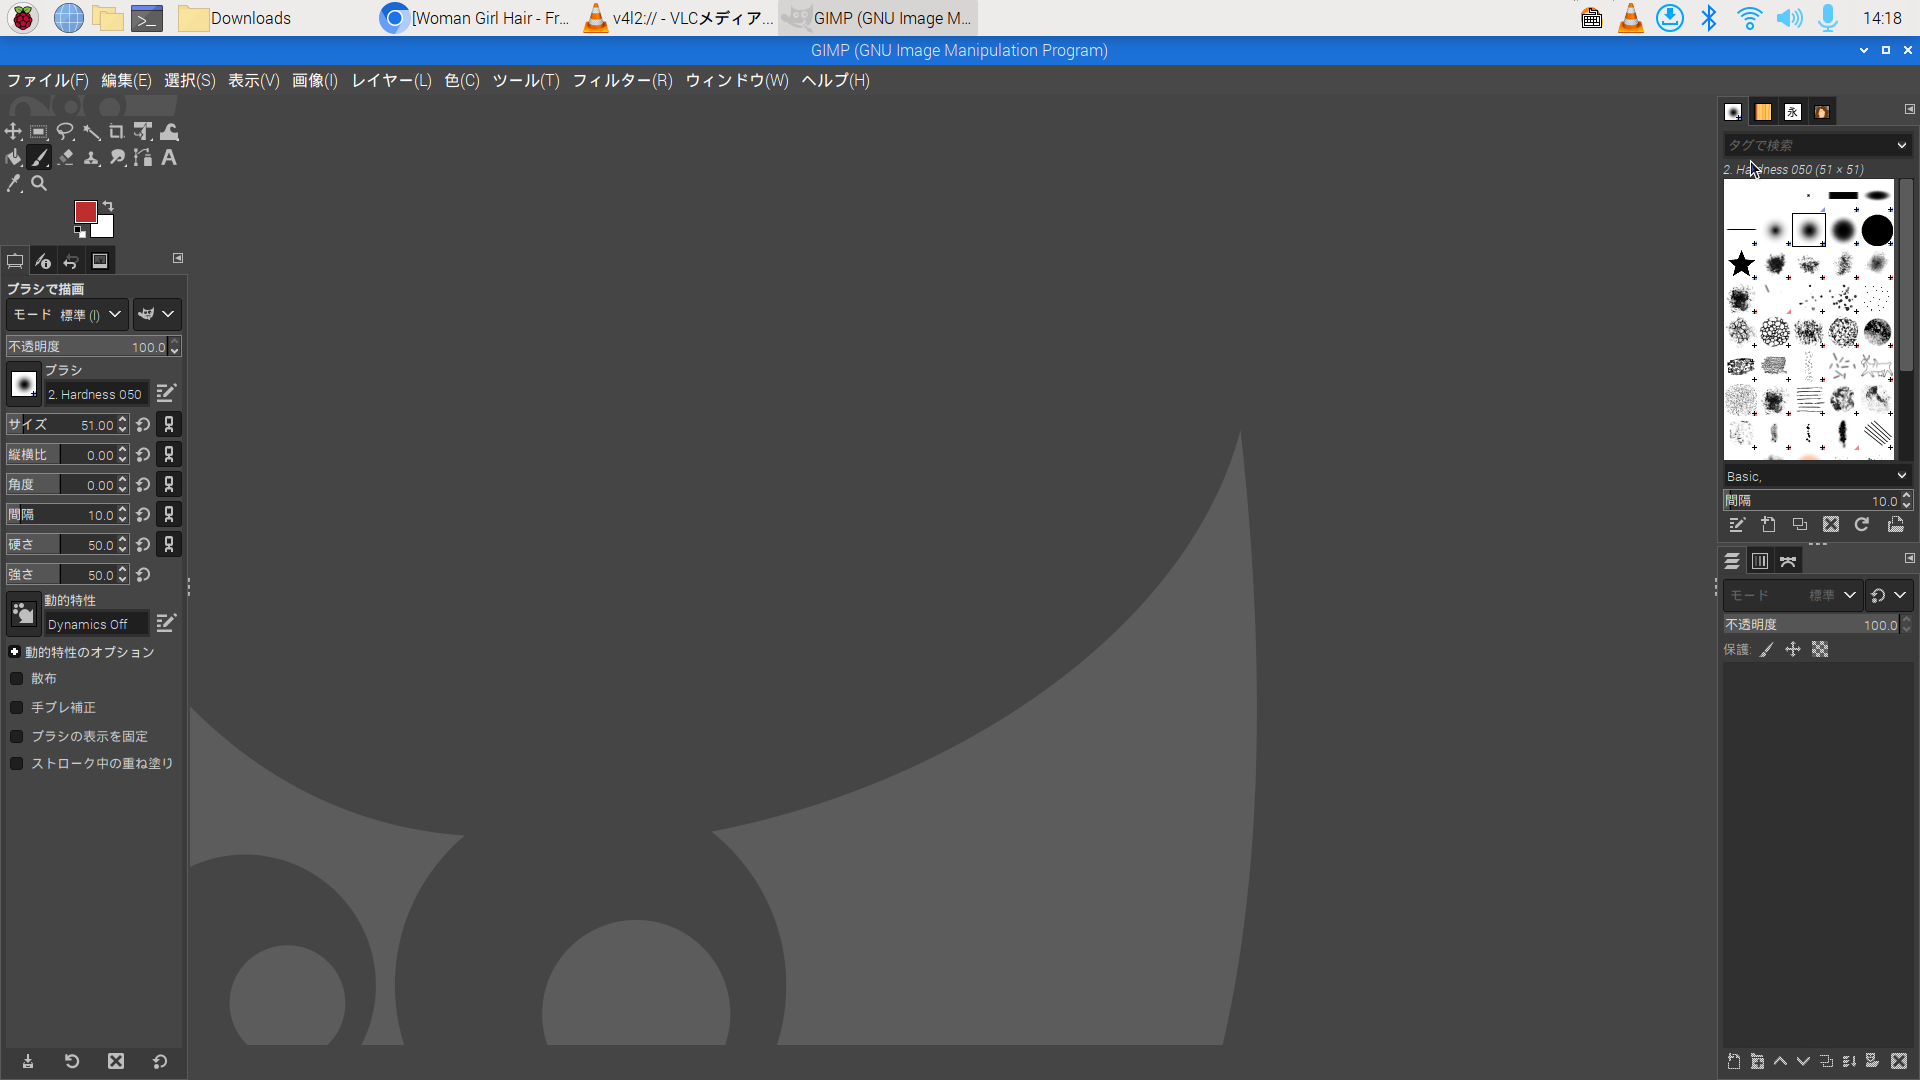
\includegraphics[width=\linewidth]{textbook-img1032.png}\\
      17 \ruby{画像}{がぞう}が消え、何もないウィンドウになります。右上の×ボタンをクリックして、\ruby{画像}{がぞう}\ruby{編集}{へんしゅう}ツールを閉じましょう
    \end{minipage}
  \end{minipage}

    \bigskip
    \begin{minipage}{0.45\linewidth}
      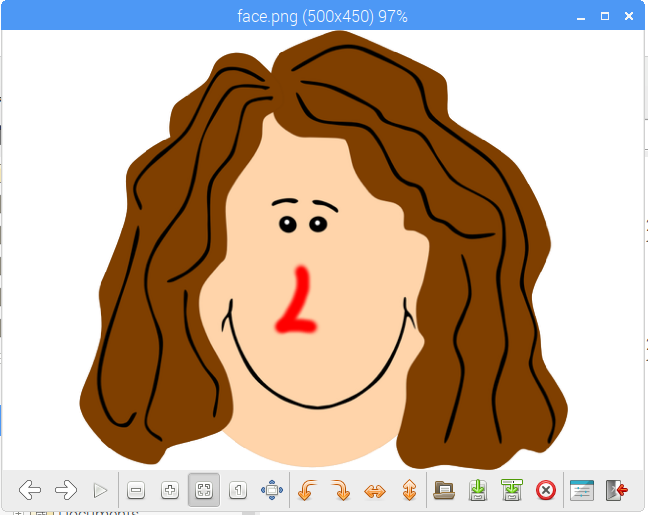
\includegraphics[width=0.9\linewidth]{textbook-img139.png}\\
      18 \ruby{画像}{がぞう}ファイルを開いて\ruby{確認}{かくにん}してみよう
    \end{minipage}

\refstepcounter{Question}\theQuestion

”GIMP”を使って、自分の顔写真をさらに\ruby{編集}{へんしゅう}、加工してみよう

  \centering
  \begin{minipage}{0.5\textwidth}
    {\upshape
      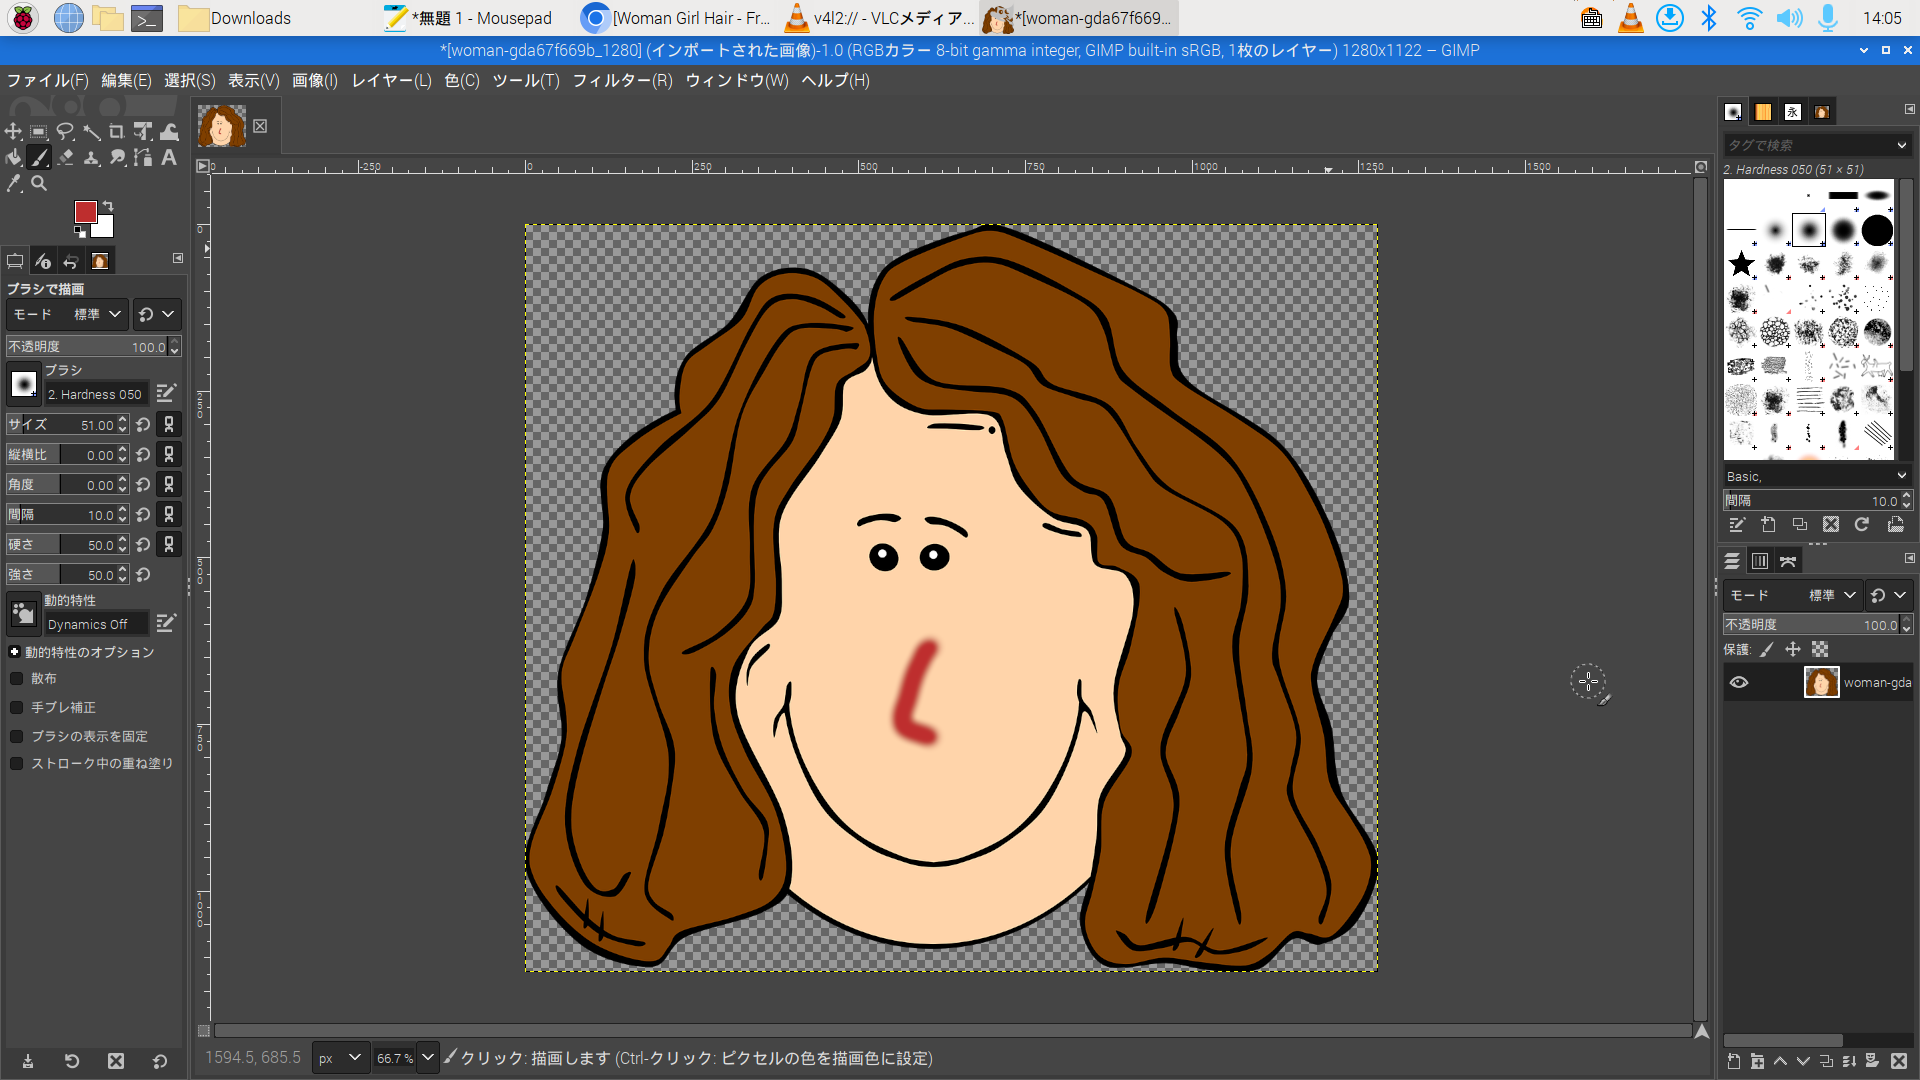
\includegraphics[width=\linewidth]{textbook-img131.png}
      \newline
      \stepcounter{Figure}{\theFigure}: GIMP\ruby{画像}{がぞう}\ruby{編集}{へんしゅう}}
  \end{minipage}
\end{figure}


\clearpage
\end{document}
